\documentclass[12pt]{article}
\usepackage[utf8]{inputenc}
\usepackage{vmargin}
\usepackage{graphicx}
\usepackage{framed, color}
\usepackage{paralist, blindtext}
\renewcommand{\contentsname}{Indice}
\renewcommand{\figurename}{Figura}
\definecolor{shadecolor}{rgb}{0.83,1,0.8}
\begin{document}

\begin{titlepage}

\newcommand{\HRule}{\rule{\linewidth}{0.5mm}} % Defines a new command for the horizontal lines, change thickness here

\center % Center everything on the page
 
%----------------------------------------------------------------------------------------
%	HEADING SECTIONS
%----------------------------------------------------------------------------------------

\textsc{\LARGE Universidad de Concepción}\\[1.5cm] % Name of your university/college
\textsc{\Large Departamento de Ingeniería Civil Informática y Ciencias de la Computación}\\[0.5cm] % Major heading such as course name
\textsc{\large Ingeniería de Software I}\\[0.5cm] % Minor heading such as course title

%----------------------------------------------------------------------------------------
%	TITLE SECTION
%----------------------------------------------------------------------------------------

\HRule \\[0.4cm]
{ \huge \bfseries Aplicación Movil en Apoyo al Turismo en la Provincia de Arauco }\\[0.4cm] % Title of your document
\HRule \\[1.5cm]
 
%----------------------------------------------------------------------------------------
%	AUTHOR SECTION
%----------------------------------------------------------------------------------------

\begin{minipage}{0.4\textwidth}
\begin{flushleft} \large
\emph{Integrantes:}\\
Cristobal \textsc{Donoso}
Matías \textsc{Medina}\\
Diego \textsc{Rodriguez}
Meraioth \textsc{Ulloa}
\end{flushleft}
\end{minipage}
~
\begin{minipage}{0.4\textwidth}
\begin{flushright} \large
\emph{Docente:} \\
Gonzalo \textsc{Rojas} % Supervisor's Name
\end{flushright}
\end{minipage}\\[4cm]

{\large \today}\\[3cm] % Date, change the \today to a set date if you want to be precise
\vfill % Fill the rest of the page with whitespace
\end{titlepage}
\tableofcontents
\newpage
%----------------------------------------------------------------------------------------
%	INTRODUCTION
%----------------------------------------------------------------------------------------
\section{Introducción}
Chile, por su geografía y diversidad climática, posee muchos lugares turísticos que yacen en el ojo de los que viajan. Sin embargo, actualmente existen lugares a pocos kilómetros de la ciudad, accesibles pero alejados en popularidad, como lo es la provincia de Arauco. Hemos escogido esta provincia dado que posee un valor cualitativo importante en el área del turismo (considerándola como una de las mayores fuentes de ingreso para la provincia) ocasionando un trade-off con el creciente avance de la gran industria.\\\\En este proyecto realizaremos un prototipo de solución el cual consiste en la creación de una aplicación móvil que ayude en la difusión, orientación y elección de puntos de interés para el turista. Se espera que esta aplicación pueda entregar un apoyo real hacia las pequeñas empresas que se encuentran registradas en el SERNATUR.\\\\Utilizaremos el proceso de desarrollo de software RUP (Proceso Racional Unificado). Esta estructura constituye una metodología de trabajo híbrida, vale decir, reúne elementos de todos los modelos de procesos genéricos. RUP consta de cuatro iteraciones entre las cuales encontramos: Inicio, Elaboración, Construcción y Transición. En el presente trabajo – y con motivos académicos – desarrollaremos hasta la fase de Construcción, mostrando un énfasis en la etapa de elaboración donde se sientan los modelos que describen el problema.\\\\Daremos inicio a nuestro informe con un Modelado de Negocio donde se representará de manera abstracta y sintetizada la organización de nuestro equipo de trabajo y su vinculación con la solución del problema. A continuación se definirán todos los requerimientos involucrados en el escenario de trabajo, los cuales han sido extraídos directamente del enunciado del problema.\\\\Dadas las condiciones que anteceden se presentará el diseño de nuestro Sistema por medio de un Diagrama de Casos de Uso y su respectiva documentación. En efecto, y dando paso a la implementación realizaremos el Diagrama de Clases UML, de Secuencia y de Comunicación, que entre otras cosas, describen el comportamiento lógico entre las clases involucradas.\\\\Finalmente, se presentarán los resultados del Sistema propuesto en su versión beta la cual no quedará ajena de posibles modificaciones en función de la evolución del Software. 
\newpage
\section{Disciplinas de RUP para la iteración}
%
%Modelado del Negocio
%
\subsection{Modelado del Negocio}
Como se ha adelantado en al sección anterior, el problema a abordar dice relación con la activación del turismo en la provincia de Arauco y con ello dar alternativas laborales a los pequeños empresarios de la zona. En consecuencia desarrollaremos un Software que atienda las necesidades de los turistas y ofusca  en el ojo del potencial cliente.\\\\Tras nuestra perspectiva y considerando la contingencia actual en el uso de aplicaciones móviles, definimos los clientes como el segmento de la población cuyas edades oscilan entre los veinticinco y cincuenta años de edad. Además buscaremos atraer al público extranjero, el cual aumentó en un 30\% este 2016 alcanzando una cifra de 720 mil personas, según informa SERNATUR [1].\\\\Actualmente yacen en el mercado otras aplicaciones las cuales forman parte de la oferta sustituta. Sin embargo, damos cuenta de la poca respuesta por parte de los clientes quienes poco utilizan las soluciones que subyacen en el área.\\\\La solución consiste en una aplicación móvil la cual podrá ser descargada desde la \emph{PlayStore} de Android. A continuación se muestra el Diagrama de Negocio que modela una búsqueda simple.
\begin{figure}[htp]
\begin{center}\centering
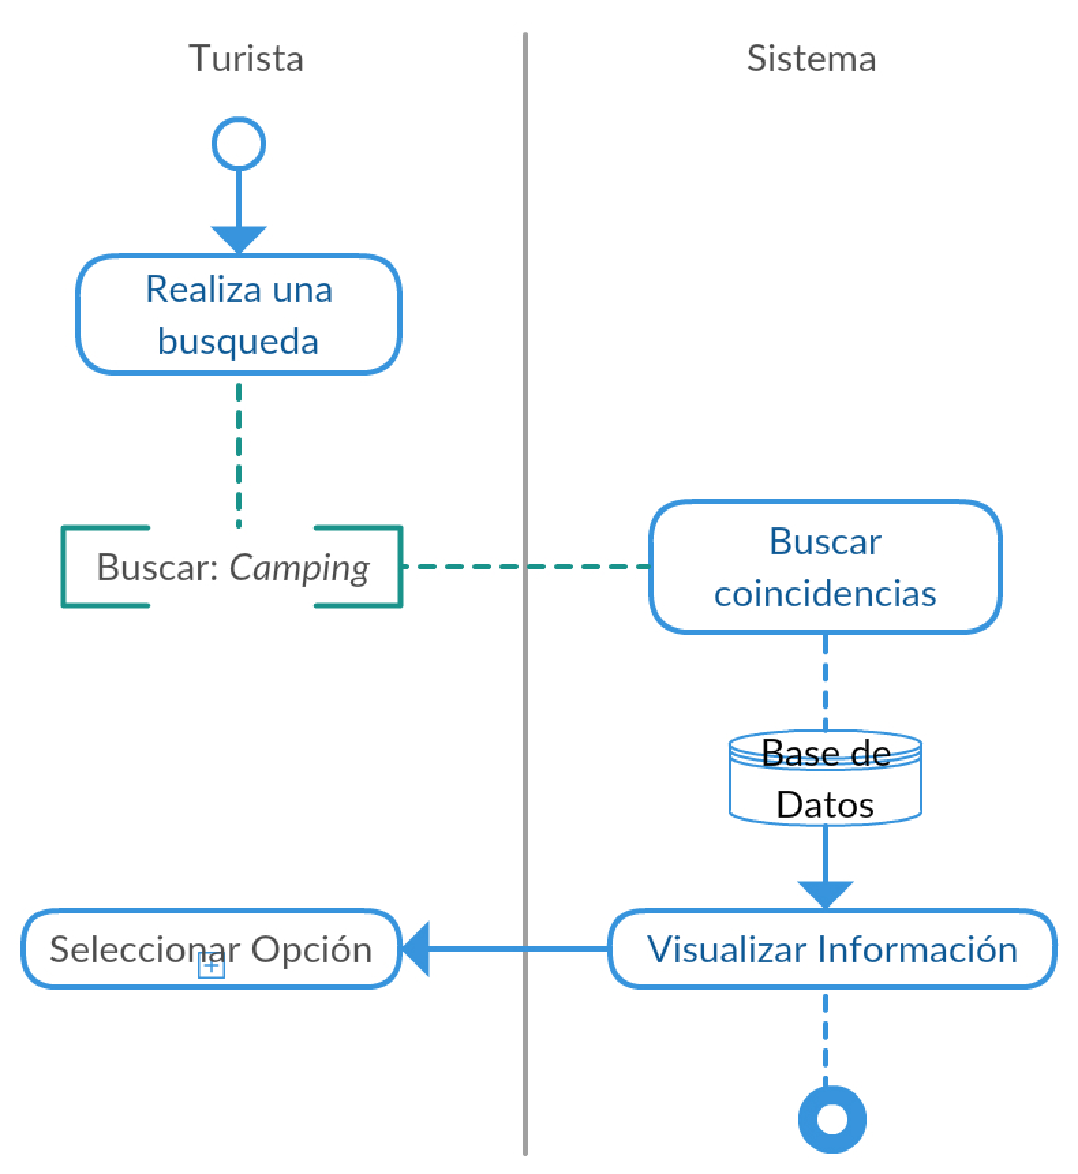
\includegraphics[scale=0.40]{/home/koskovi/Documentos/IS/Don-Oso/Informe/MN.pdf}
\caption{Diagrama de Modelo de Negocio asociado a la búsqueda}
\label{}\end{center}
\end{figure}
%%
%%requerimientos
%%
\subsection{Requerimientos}
A partir del enunciado del problema se extrajo los distintos requerimientos que debe cumplir el sistema, éstos son:
\begin{enumerate}
\item Mantener información de las sucursales junto con sus distintos servicios y a que empresa está asociado.
\item Obtener información adicional o modificar la existente desde los empresarios sobre sus propias sucursales y servicios.
\item Categorizar servicios de las distintas sucursales en el momento de agregar dicho servicio al sistema. Las categorías y sub-categorías vienen predefinidas en el sistema.
\item Indicar dentro de la aplicación si un Empresario cuenta con el sello de turistmo sustentable.
\item Buscar servicios registrados por medio de distintos criterios:
	\begin{itemize}
		\item Nombre Servicio.
		\item Punto de interés.
		\item Sucursal.
		\item Categoría.
		\item Sub-Categoría.
	\end{itemize}
\item Enriquecer información existente sobre una sucursal por medio experiencia de turistas, estas son:
	\begin{itemize}
		\item Comentarios
		\item Evaluación de distintos criterios.
		\item Indicaciones y consejos de orientación a una sucursal.
	\end{itemize}
\item Crear un sistema de 
\item Rutas a servicios.
\newpage
\item Facilitar indicaciones a punto de interés de difícil acceso. mediante:
	\begin{itemize}
		\item Indicaciones con fotografía de hitos y referencias conocidas.
		\item Información de buses urbanos o lugares.
		\item Consejos de orientación proporcionada por
	\end{itemize}
\item Proveer mapa turístico de oferta turística categorizada.
\item Permitir a los turistas:
	\begin{itemize}
		\item Crear itinerario.
		\item Buscar itinerarios.
		\item Comentar itinerario.
		\item Borrar itinerario.
		\item Compartir itinerario en redes sociales externas.		
	\end{itemize}
\end{enumerate}
\newpage
%
%Análisis y Diseño
%
\subsection{Análisis y Diseño	} 
De los requerimientos previamente listados, se ha elaborado el siguiente diagrama de casos de uso, el cual muestra cuales son los actores involucrados en el sistema y los distintos casos de uso que éstos pueden llevar a cabo.
\begin{figure}[htp]
\centering
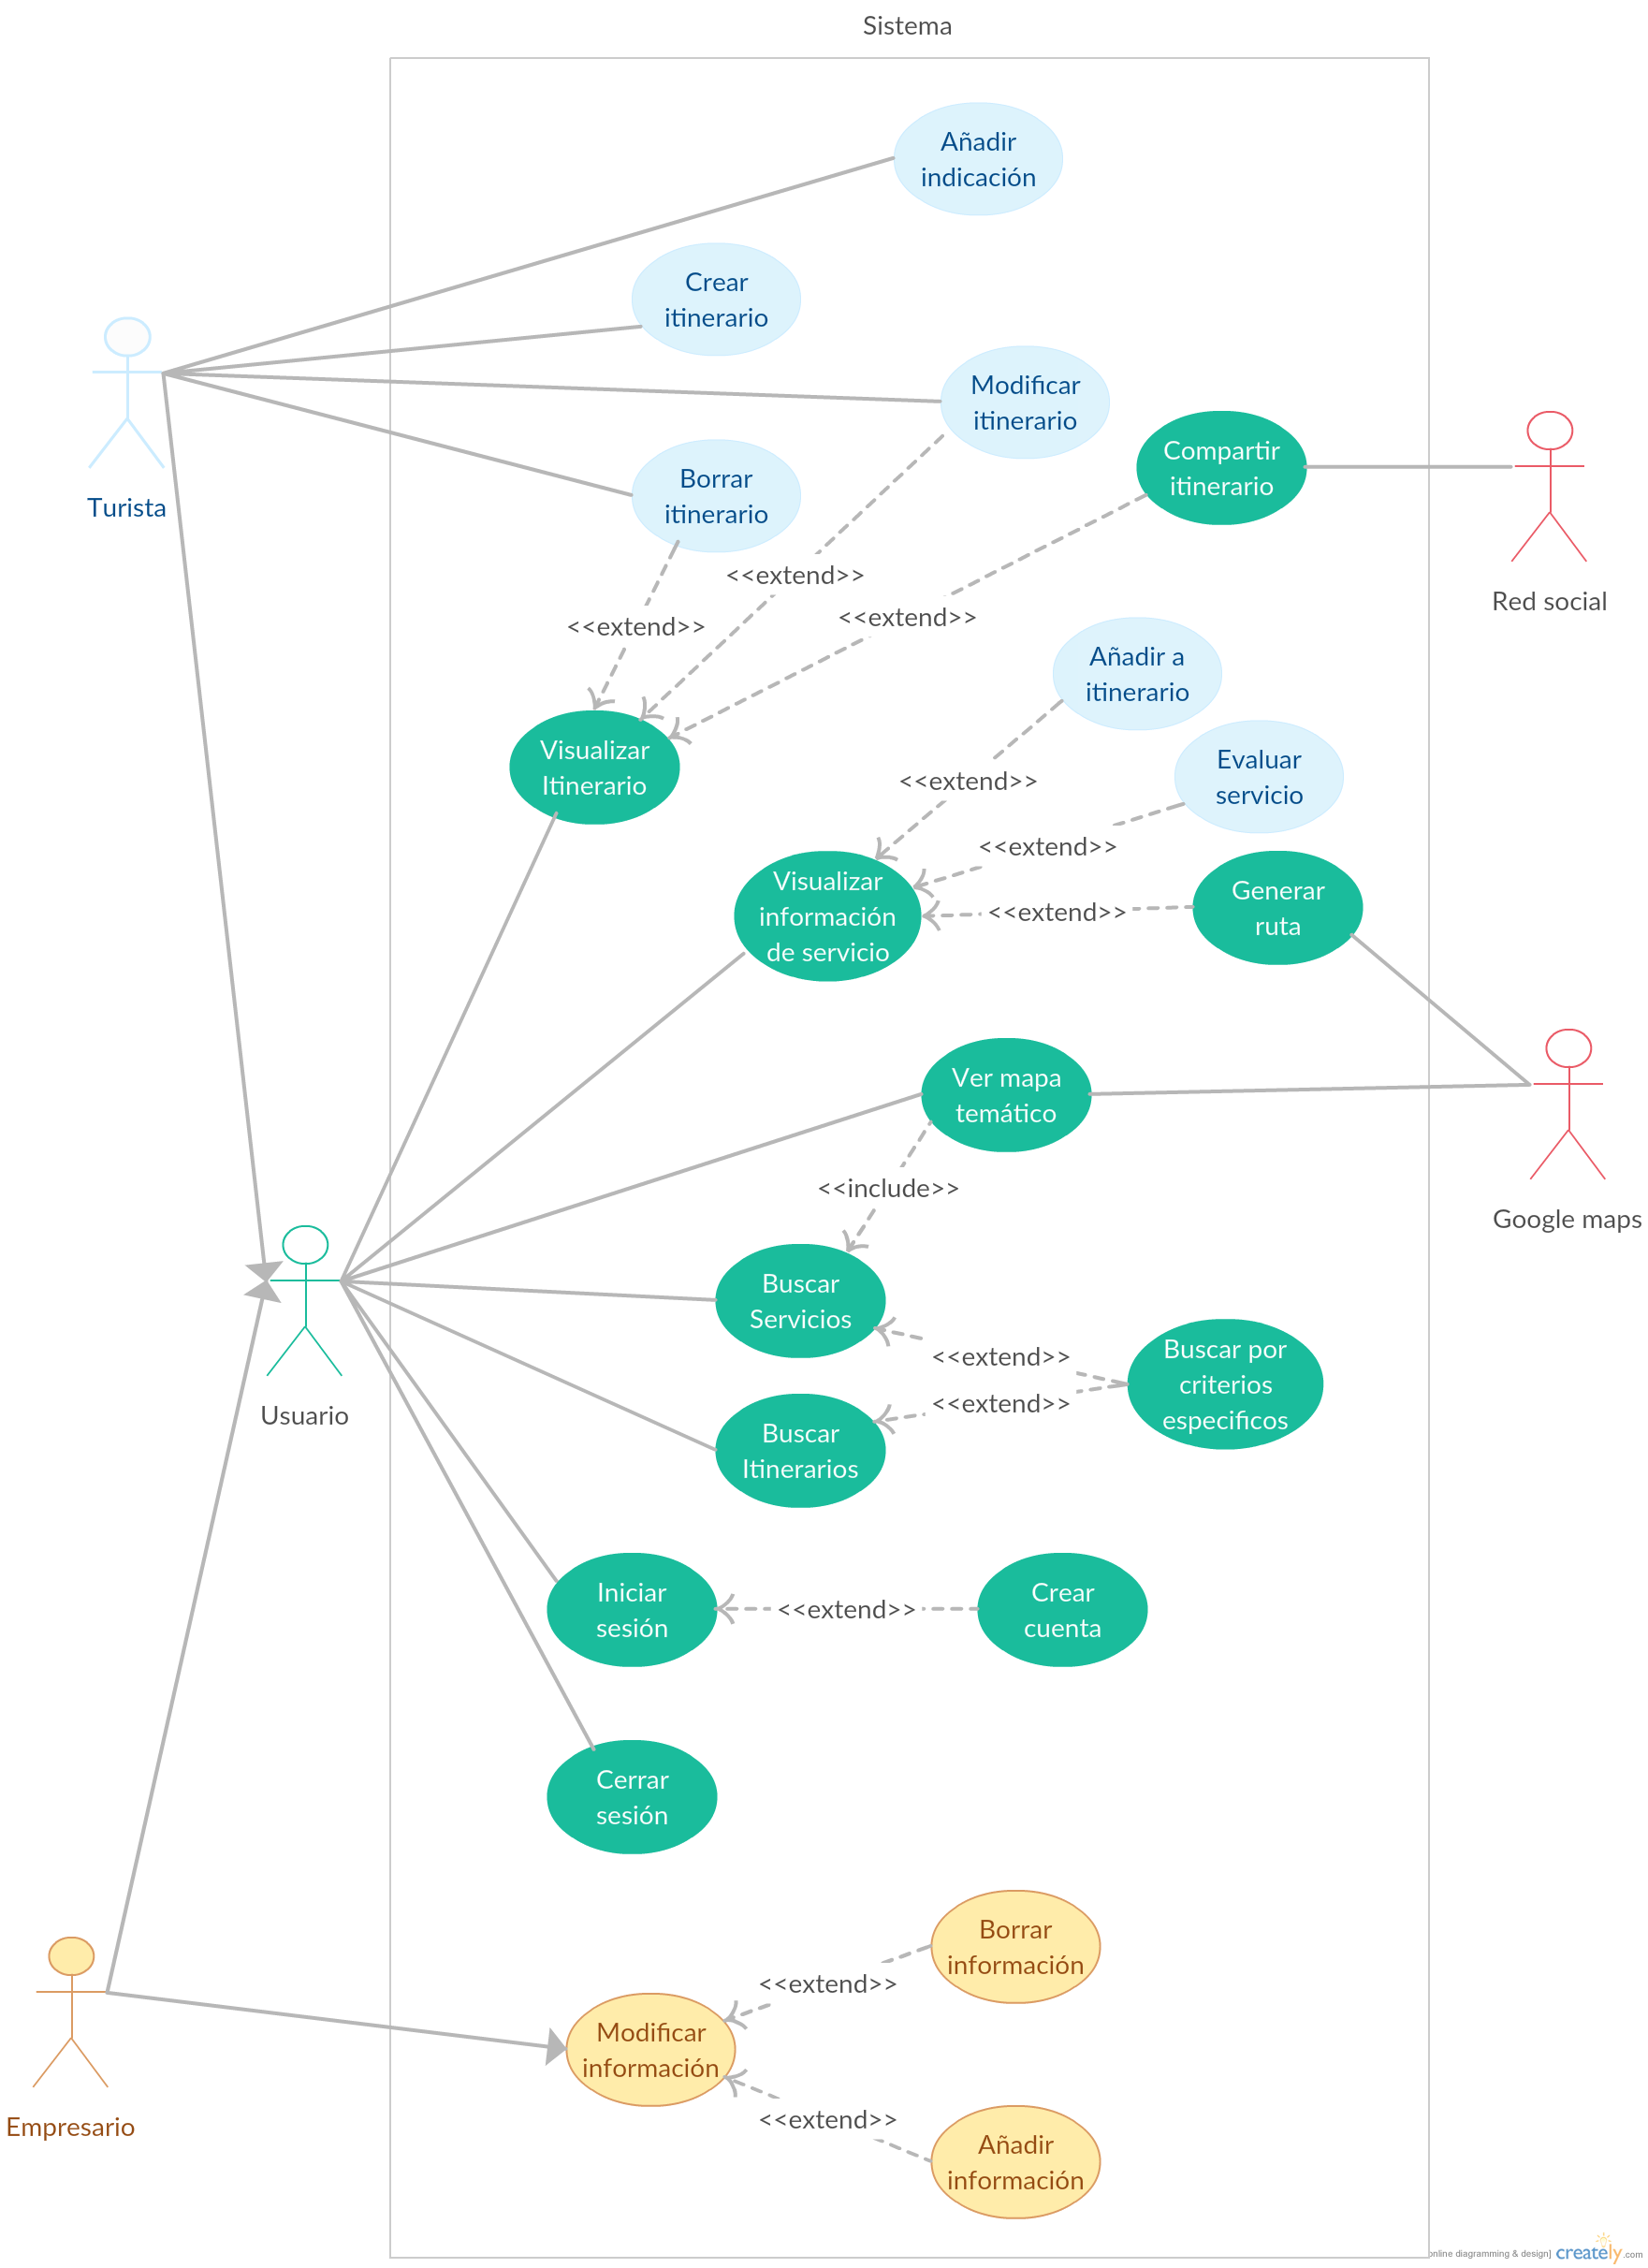
\includegraphics[scale=0.20]{Informe/cu.png}
\caption{Diagrama de Casos de Uso}
\label{}
\end{figure}
%
%Documentacion
%
\section{Documentación Casos de Uso}
Para esta iteración, y conforme a cumplir los requerimientos acordados en un principio, se modificaron e implementaron los siguientes casos de uso:

\subsection{\textbf{CASO DE USO UC1:} Ver mapa temático }
\textbf{Actor principal:} Usuario\\
\\
\textbf{Personal involucrado e intereses: }\\
\underline{Usuario:} Quiere visualizar un mapa de sucursales que tengan ciertos servicios.\\\underline{Google Maps:} Quiere recibir peticiones de PoI para mostrar en mapa de forma correcta.\\
\\
\textbf{Precondiciones:} El usuario apretó el botón de mapa temático\\
\\
\textbf{Postcondiciones:} El usuario visualiza un mapa (geográfico) con marcas donde se encuentran las sucursales que contienen los servicios que está buscando.\\
\\
\textbf{Escenario principal de éxito:}
\begin{enumerate}
\item Se envía una petición a Google Maps para proveer el mapa de la provincia de Arauco.
\item El usuario visualiza el mapa
\item El sistema invoca al caso de uso \textbf{Busar Servicios (UC2)}, lo que permite obtener una lista con sucursales filtrada.
\item Se envía una petición a Google Maps para que ubique las sucursales listadas en el mapa.
\item Las sucursales aparecen en el mapa.
\end{enumerate}
\textbf{Excepciones:}
\begin{enumerate}
\item[1-4'] Falla conexión con Google Maps, se muestra un mensaje de error.
\item[1-5'] El turista apreta cancelar.
\end{enumerate}
\newpage
\subsection{\textbf{CASO DE USO UC2:} Buscar sucursales }
\textbf{Actor principal:} Usuario\\
\\
\textbf{Personal involucrado e intereses: }\\\underline{Usuario:} Quiere encontrar sucursales que contenga servicios que busca.\\
\\
\textbf{Precondiciones:} El usuario necesita una lista filtrada de sucursales.\\
\\
\textbf{Postcondiciones:} EL usuario obtiene una lista de sucursales.\\
\\
\textbf{Escenario principal de éxito:}
\begin{enumerate}
\item El usuario apreta el botón de busqueda de servicios.
\item El usuario ingresa un valor en el campo de búsqueda.
\item El sistema busca sucursals con tipos de servicios acorde al campo de búsqueda ingresa.
\item Se muestra al usuario una lista con sucursales.
\end{enumerate}
\textbf{Excepciones:}
\begin{enumerate}
\item[2'a] El usuario cancela la operación.
\item[2'b] El usuario puede apretar el botón de busqueda con criterios específicos. El sistema invoca al caso de uso \textbf{Buscar por criterios específicos (UC3)}.
\item[4'] Lista vacía, se informa que no se encontró lo que el usuario buscaba.
\end{enumerate}
\newpage
\subsection{\textbf{CASO DE USO UC3:} Buscar por criterios específicos }
\textbf{Actor principal:} Usuario\\
\\
\textbf{Personal involucrado e intereses: }\\\underline{Usuario:} Quiere extender su busqueda de iteraciones o sucursales con mayor criterio de busqueda.
\\\\
\textbf{Precondiciones:}El usuario estaba buscando sucursales o itinerarios en el sistema, se informa que tipo de busqueda es.\\ 
\\
\textbf{Postcondiciones:} El usuario obtiene una lista con sucursales o itinerarios que cumplen con los criterios específicos.\\
\\
\textbf{Escenario principal de éxito:}
\begin{enumerate}
\item El usuario selecciona de una lista el/los criterios de busqueda que desea.
\item El usuario ingresa un valor de busqueda por cada criterio seleccionado.
\item El sistema busca los sucursales o itinerarios acorde al campo de búsqueda.
\item Se muestra al usuario una lista con sucursales o itinerarios.
\end{enumerate}
\textbf{Excepciones:}
\begin{enumerate}
\item[2'] El usuario puede cancelar la interacción.
\item[4'] Lista vacía, se informa que no se encontró lo que el usuario buscaba.
\end{enumerate}
\newpage
\subsection{\textbf{CASO DE USO UC4:} Buscar itinerarios }
\textbf{Actor principal:} Usuario\\
\\
\textbf{Personal involucrado e intereses: }\\\underline{Usuario} Quiere encntrar el/los itinerario/s que cumplan con su criterio de busqueda.\\
\\
\textbf{Precondiciones:} El usuario necesita una lista de itinerarios.\\
\\
\textbf{Postcondiciones:} El usuario obtiene una lista de itinerarios.\\
\\
\textbf{Escenario principal de éxito:}
\begin{enumerate}
\item Usuario apreta botón de búsqueda de itinerario.
\item Usuario ingresa valor en campo de búsqueda.
\item El sistema busca itinerarios acorde al campo de búsqueda.
\item Se muestra al usuario una lista con itinerarios.
\end{enumerate}
\textbf{Excepciones:}
\begin{enumerate}
\item[2'a] El usuario cancela la operación.
\item[2'b] El usuario puede apretar el botón de busqueda con criterios específicos. El sistema invoca al caso de uso \textbf{Buscar por criterios específicos (UC3)}.
\end{enumerate}
\newpage
\subsection{\textbf{CASO DE USO UC5:} Visualizar información de sucursal }
\textbf{Actor principal:} Usuario y Turista\\
\\
\textbf{Personal involucrado e intereses: }\\\underline{Usuario y Turista:} Quiere ver información asociada a una sucursal.\\
\\
\textbf{Precondiciones:} El usuario ha seleccionado una sucursal, ya sea desde busqueda, itinerario o mapa temático.\\
\\
\textbf{Postcondiciones:} El usuario ve en pantalla la información relevante de la sucursal.\\
\\
\textbf{Escenario principal de éxito:}
\begin{enumerate}
\item El sistema obtiene la información de la sucursal.
\item El sistema muestra la información al usuario.
\end{enumerate}
\textbf{Excepciones:}
\begin{enumerate}
\item[3'a] El turista apreta el botón de evaluar servicios, el sistema invoca al caso de uso \textbf{Evaluar Servicios (UC6)}. 
\item[3'b] El turista apreta el botón de añadir a itinerario, el sistemainvoac al caso de uso \textbf{Añadir a itinerario (UC7)}.
\item[3'c] El usuario apreta el botón de generar ruta, el sistema invoca al caso de uso \textbf{Generar ruta (UC8)}.
\item[3'd] El usuario apreta el botón de evaluar servicios o el botón de añadir a itinerario. Se muestra un mensaje de error por no iniciar sesión.
\end{enumerate}
\newpage
\subsection{\textbf{CASO DE USO UC6:} Evaluar servicio }
\textbf{Actor principal:} Turista\\
\\
\textbf{Personal involucrado e intereses: }\\\underline{Turista:} Desea evaluar servicios de una sucursal.
\\
\textbf{Precondiciones:} El turista se encuentra visualizando una sucursal.\\
\\
\textbf{Postcondiciones:} El turista ha evaluado los servicios que quería de una sucursal.\\
\\
\textbf{Escenario principal de éxito:}
\begin{enumerate}
\item El sistema muestra una lista de seriicios de la sucursa con estrellas sin nota o con nota si ya se había evaluado.
\item El turista selecciona cuantas estrellas le asigna a cada servicio que quiera.
\item El turista finaliza al presionar botón de evaluar.
\end{enumerate}
\textbf{Excepciones:}
\begin{enumerate}
\item[2'] El turista modifica una evaluación hecha previamente.
\item[1-3'] Turista Cancela.
\end{enumerate}

\subsection*{\textbf{CASO DE USO UC7:} Añadir a Itinerario }
\textbf{Actor principal:} Turista\\
\\
\textbf{Personal involucrado e intereses: }\\
\underline{Turista}: Desea añadir servicios a un itinerario creado por él.
\\\\
\textbf{Precondiciones:} El turista se encuentra visualizando una sucursal desde una lista o su detalle.\\
\\
\textbf{Postcondiciones:} El turista añade servicio(s) de una sucursal a un itinerario.\\
\\
\textbf{Esecnario principal de éxito:}
\begin{enumerate}
\item El turista selecciona en orden los servicios que desea agregar.
\item El turista apreta el botón agregar a itinerario.
\item EL sistema muestra una lista con itinerarios del turista.
\item El turista selecciona el itinerario al cual desea agregar servicios.
\item Finaliza apretando OK.
\end{enumerate}
\textbf{Excepciones:}
\begin{enumerate}
\item[1-5'] Cancelar.
\end{enumerate}

\subsection{\textbf{CASO DE USO UC8:} Generar Ruta }
\textbf{Actor principal:} Usuario\\
\\
\textbf{Personal involucrado e intereses:}\\
\underline{Usuario}: Desea ver una ruta a una sucursal.\\
\underline{Google Maps}: Quiere recibir peticiones de ruta entre dos puntos en el mapa.
\\\\
\textbf{Precondiciones:} Usuario se encuentra visualizando sucursal desde una lista o el detalle y tiene activado el GPS.\\
\\
\textbf{Postcondiciones:} Usuario ve ruta desde su posición hasta una sucursal.\\
\\
\textbf{Esecnario principal de éxito:}
\begin{enumerate}
\item El usuario ingresa qué tipo de transporte utilizará.
\item Se envía información a MAPS junto con posición del usuaro, posición de sucursal y el medio de transporte.
\item MAPS entrega un mapa de la ruta.
\item El sistema muestra la información al usuario.
\end{enumerate}
\textbf{Excepciones:}
\begin{enumerate}
\item[2'] Falla la conexión con MAPS, se muestra una alerta.
\item[3'] No existe ruta, se entrega un mensaje de error.
\end{enumerate}
\newpage
\subsection{\textbf{CASO DE USO UC9:} Visualizar Itinerario }
\textbf{Actor principal:} Usuario, Turista\\
\\
\textbf{Personal involucrado e intereses: }\\
\underline{Usuario}: quiere visualizar los contenidos de un itinerario.\\
\underline{Turista}: puede visualizar el contenido de un itinerario y compartirlo. Además puede modificar o borrar itinerarios creados por él.
\\\\
\textbf{Precondiciones:} El usuario está visualizando una lista de itinerarios, por ejemplo después del caso de uso "buscar itinerario".\\
\\
\textbf{Postcondiciones:} El sistema muestra al usuario los detalles contenidos en un itinerario.\\
\\
\textbf{Esecnario principal de éxito:}
\begin{enumerate}
\item El usuario selecciona un itinerario de la lista de itinerarios.
\item El usuario selecciona la opción de visualización de contenido.
\item El sistema muestra la información detallada del itinerario.
\end{enumerate}
\textbf{Excepciones:}
\begin{enumerate}
\item[2'] El usuario deselecciona el itinerario y no se visualiza el contenido.
\item[3'a] El turista puede seleccionar la opción borrar y se salta al caso de uso "Borrar itinerario (CU10)".
\item[3'b] El turista puede seleccionar la opción modificar y se salta al caso de uso "Modificar itinerario (CU11)".
\item[3'c] El turista puede seleccionar la opción compartir y se salta al caso de uso "Compartir itinerario (CU12)".
\end{enumerate}

\newpage
\subsection{\textbf{CASO DE USO UC10: Borrar Itinerario}  }
\textbf{Actor principal:} Turista.\\
\\
\textbf{Personal involucrado e intereses: }\\
\underline{Turista}:Quiere eliminar un itinerario creado por él.
\\\\
\textbf{Precondiciones:} El turista ha seleccionado la opcion borrar itinerario desde la visualización de su itinerario.\\
\\
\textbf{Postcondiciones:} Se elimina el itinerario seleccionado de la base de datos.\\
\\
\textbf{Esecnario principal de éxito:}
\begin{enumerate}
\item El turista selecciona la opción de borrar itinerario.
\item Se elimina el itinerario seleccionado de la base de datos.
\end{enumerate}
\textbf{Excepciones:}
\begin{enumerate}
\item[1'] El turista puede cancelar la eliminación de su itinerario.
\end{enumerate}



\subsection{\textbf{CASO DE USO UC11: Modificar Itinerario}  }
\textbf{Actor principal:} Turista.\\
\\
\textbf{Personal involucrado e intereses: }\\
\underline{Turista}:Quiere eliminar servicios contenidos en su itinerario o cambiar el orden de éstos.
\\\\
\textbf{Precondiciones:} El turista ha seleccionado la opcion modificar itinerario desde la visualización de su itinerario.\\
\\
\textbf{Postcondiciones:} Se modifica el contenido del itinerario.\\
\\
\textbf{Esecnario principal de éxito:}
\begin{enumerate}
\item El turista selecciona la opción de modificar itinerario.
\item El turista selecciona un servicio dentro del itinerario.
\item El turista selecciona otro servicio dentro del itinerario y se intercambian en el orden.
\end{enumerate}
\textbf{Excepciones:}
\begin{enumerate}
\item[3'a] El turista selecciona la opción borrar servicio para borrar el servicio seleccionado del itinerario.
\item[1-3'] El turista puede salir en cualquier momento del modo edición.
\end{enumerate}


\newpage
\subsection{\textbf{CASO DE USO UC12: Compartir Itinerario}  }
\textbf{Actor principal:} Turista.\\
\\
\textbf{Personal involucrado e intereses: }\\
\underline{Turista}:Quiere compartir un itinerario en redes sociales.
\\\\
\textbf{Precondiciones:} El turista está visualizando una lista de itinerarios, por ejemplo después del caso de uso "buscar itinerario" o está visualizando el contenido de un itinerario.\\
\\
\textbf{Postcondiciones:} El turista publica en la red social elegida el itinerario seleccionado.\\
\\
\textbf{Esecnario principal de éxito:}
\begin{enumerate}
\item El turista selecciona un itinerario de la lista de itinerarios.
\item El turista selecciona la opción compartir itinerario y selecciona dónde compartirlo.
\item Se abre la opción de compartir de la red social elegida.
\item Se comparte satisfactoriamente el itinerario seleccionado.
\end{enumerate}
\textbf{Excepciones:}
\begin{enumerate}
\item[2-3'] El turista puede cancelar la acción en todo momento.
\item[3']s Error al conectar con la red social, se cancela la acción.
\end{enumerate}
\newpage
\subsection{\textbf{CASO DE USO UC13:} Crear itinerario }

\textbf{Actor principal:} Turista\\
\\
\textbf{Personal involucrado e intereses: }\\\underline{Turista:} Quiere crear un itinerario en la aplicación.\\
\\
\textbf{Precondiciones:} El turista, desde sus itinerarios, accede a la creación de itinerarios.\\
\\
\textbf{Postcondiciones:} El turista crea un itinerario vacío.\\
\\
\textbf{Escenario principal de éxito:}
\\
\begin{enumerate}
\item El turista escribe el nombre del nuevo itinerario.
\item Si el nombre no se repite con otro, se crea el nuevo itinerario.
\end{enumerate}
\textbf{Excepciones:}
\begin{enumerate}
\item[1-2'] Cancelar: En cualquier momento el turista puede cancelar la operación.
\item[2'] El nombre del itinerario ya existe. Se emite un mensaje y se vuelve al paso 1.
\end{enumerate}
\section{Diagrama de Clases UML}
Previo a la implementación es necesario modelar cuales serán los elementos presentes en la base de datos utilizada por el sistema. Basándonos en los casos de uso de la sección anterior, se presenta a continuación el diagrama de clases de la base de datos.\\
\begin{figure}[htp]
\centering
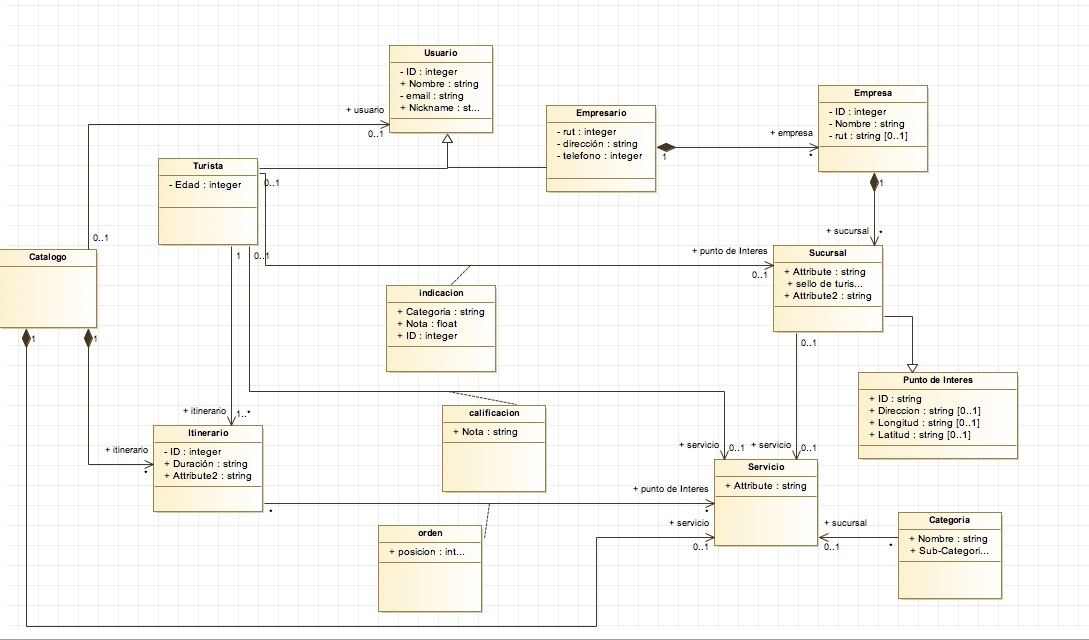
\includegraphics[scale=0.6, angle=90]{Informe/dcfinal.png}
\caption{Diagrama de Clases UML}
\label{}
\end{figure}
\newpage
\subsection{Implementación}
A partir del diagrama de clases anterior, generamos el siguiente modelo relacional para nuestra base de datos, el cual posteriormente fue implementado en MySQL.
\subsubsection{Modelo Relacional}
\textbf{USUARIO} (\underline{ID}, Nombre, E-mail) PK: ID\\\\
\textbf{EMPRESARIO} (\underline{ID}, RUT, Dirección, teléfono) PK: ID; FK: ID FROM USUARIO(ID)\\\\
\textbf{TURISTA} (\underline{ID}, Edad) PK: ID ; FK: ID FROM USUARIO(ID)\\\\
\textbf{EMPRESA} (\underline{ID}, Nombre, RUT\_Empresa, ID\_Empresario) PK: ID, FK: ID\_Empresario FROM EMPRESARIO(ID)\\\\
\textbf{PUNTO\_DE\_INTERES} (\underline{ID}, Dirección, Longitud) PK: ID\\\\
\textbf{SUCURSAL} (\underline{ID\_POI},Nombre, Sello de turismo, ID\_Empresa) PK: ID\_POI, FK: ID\_Empresa FROM EMPRESA(ID), ID\_POI FROM PUNTO\_DE\_INTERES(ID)\\\\
\textbf{LUGAR DE LIBRE ACCESO} (\underline{ID\_POI}, Nombre) PK: ID\_POI , FK: ID\_POI FROM PUNTO\_DE\_INTERES(ID)\\\\
\textbf{SERVICIO} (\underline{Nombre\_Servicio}, ID\_POI) PK: Nombre\_Servicio , FK: ID\_POI FROM SUCURSAL(ID\_POI)\\\\
\textbf{CATEGORIA} (\underline{Nombre\_Categoria}) PK: Nombre\_Categoría\\\\
\textbf{CATEGORIA\_SUCURSAL} (\underline{ID\_POI}, \underline{Nombre\_Categoría}) PK: ID\_POI, Nombre\_Categoría , PK: ID\_POI FROM SUCURSAL(ID\_POI), Nombre\_Categoria FROM CATEGORIA(Nombre\_Categoria)\\\\
\textbf{INDICACION} (\underline{ID}, Texto, ID\_POI) PK: ID, FK: ID\_POI FROM PUNTO\_DE\_INTERES(ID)\\\\
\textbf{ITINERARIO} (\underline{ID}, Duración, ID\_Usuario), PK: ID, FK: ID\_Usuario FROM USUARIO(ID)\\\\
\textbf{ORDEN} (\underline{ID\_Itinerario}, \underline{ID\_POI}, \underline{Posicion}) PK: ID\_Itinerario, ID\_POI, Posicion, FK: ID\_Itinerario FROM ITINERARIO(ID), ID\_POI FROM PUNTO\_DE\_INTERES(ID)\\\\
\textbf{CALIFICACION} (\underline{ID}, \underline{ID\_Turista}, \underline{ID\_POI}, Categoria, Nota) PK: ID, ID\_Turista, ID\_POI , FK: ID\_Turista FROM TURISTA (ID), ID\_POI FROM PUNTO\_DE\_INTERES (ID)
\subsubsection{Base de datos en MySQL}
A continuación se muestran algunas tablas de la base de datos. Son capturas de pantalla de la consola de mysql.\\
\begin{figure}[htp]
\centering
\begin{flushleft}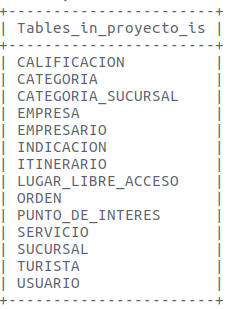
\includegraphics[scale=0.50]{Informe/bd10.png}\end{flushleft}
\begin{flushleft}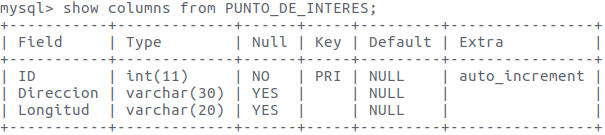
\includegraphics[scale=0.50]{Informe/bd11.png}\end{flushleft}
\begin{flushleft}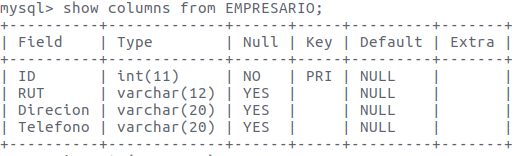
\includegraphics[scale=0.50]{Informe/bd12.png}\end{flushleft}
\caption{Tablas sql generadas desde terminal}
\label{}
\end{figure}
\newpage
%%%%%%%%%%%%%%%%%%%%%%%%TESTING%%%%%%%%%%%%%%%%%%%%%%%%%%%%%%%%%%%%%%%
\subsection{Testing}
Hasta el momento hemos agregado información a tres tablas de la base de datos, USUARIO, TURISTA y EMPRESARIO, es decir contamos con información de personas que usarán la aplicación.\\\\
Los datos agregados son generados al azar automáticamente con la herramienta "\emph{generatedata}" encontrada online.\\\\
A continuación se muestra una captura de pantalla de la consola de mysql con la consulta que retorna aquellos usuarios turistas con edad entre 18 y 45 años.\\
\begin{figure}[htp]
\centering
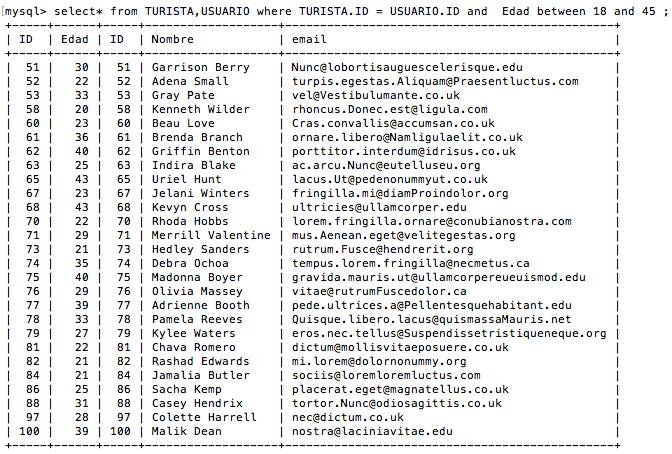
\includegraphics[scale=0.60]{Informe/bd2.jpg}
\caption{Consulta sql}
\label{}
\end{figure}
\section{Diagramas de Secuencia}
A continuación mostraremos alguno de los Casos de Uso que fueron elegidos para ser implementados en la versión beta de nuestra aplicación.
\newpage
\subsection{Añadir Información}
\begin{center}\begin{figure}[htp]
\centering
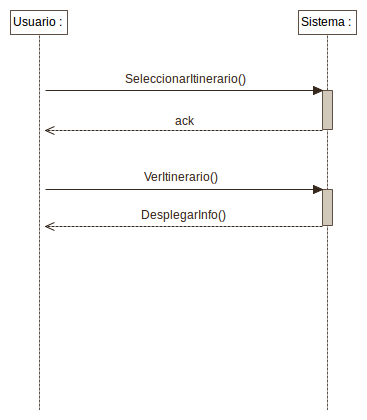
\includegraphics[scale=0.50]{Diagramas/Secuencia/visualizar_itinerario.png}
\caption{Diagrama de Secuencia para CU Visualizar Itinerario}
\label{}
\end{figure}\end{center}
\subsection{Busqueda de Itinerario}
\begin{center}\begin{figure}[htp]
\centering
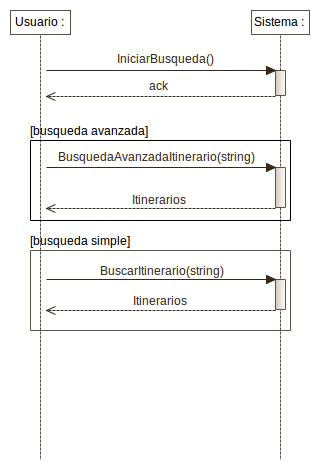
\includegraphics[scale=0.45]{Diagramas/Secuencia/busqueda_itinerario.png}
\caption{Diagrama de Secuencia para CU Buscar Itinerario}
\label{}
\end{figure}\end{center}
\newpage
\subsection{Busqueda de Servicio}
\begin{center}\begin{figure}[htp]
\centering
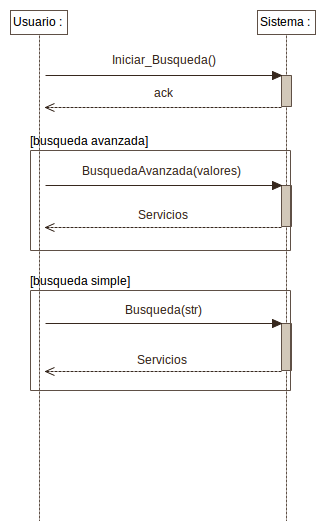
\includegraphics[scale=0.50]{Diagramas/Secuencia/busqueda_servicio.png}
\caption{Diagrama de Secuencia para CU Buscar Servicio }
\label{}
\end{figure}\end{center}
\subsection{Calificar}
\begin{figure}[htp]
\centering
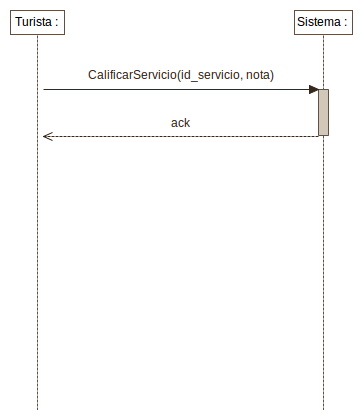
\includegraphics[scale=0.41]{Diagramas/Secuencia/calificar.png}
\caption{Diagrama de Secuencia para CU Calificar Servicio}
\label{}
\end{figure}
\newpage
\subsection{Crear Itinerario}
\begin{figure}[htp]
\centering
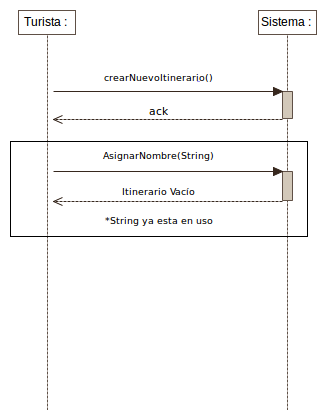
\includegraphics[scale=0.50]{Diagramas/Secuencia/crear_itinerario.png}
\caption{Diagrama de Secuencia para CU Crear Itinerario}
\label{}
\end{figure}
\subsection{Visualizar Información de Servicio}
\begin{figure}[htp]
\centering
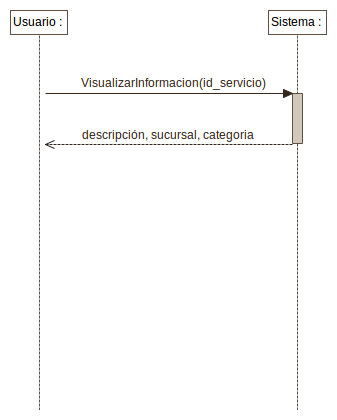
\includegraphics[scale=0.50]{Diagramas/Secuencia/visualizar_info_servicio.png}
\caption{Diagrama de Secuencia para CU Visualizar Información de Servicio}
\label{}
\end{figure}
\newpage
\subsection{Visualizar itinerario}
\begin{figure}[htp]
\centering
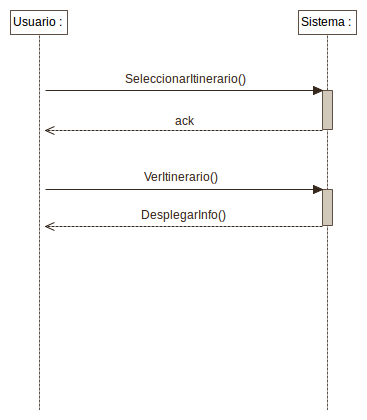
\includegraphics[scale=0.60]{Diagramas/Secuencia/visualizar_itinerario.png}
\caption{Diagrama de Secuencia para CU Visualizar Itinerario}
\label{}
\end{figure}
%
%Diagramas de comunicación
%
\section{Diagramas de Comunicación}
A continuación procedemos a mostrar los respectivos diagramas de comunicación correspondiente a los casos de uso seleccionados en la sección anterior. Para cada uno de los diagramas de comunicación considere el flujo de izquierda a derecha y de arriba a abajo.
\subsection{Visualizar Información del Servicio}
\begin{figure}[htp]
\centering
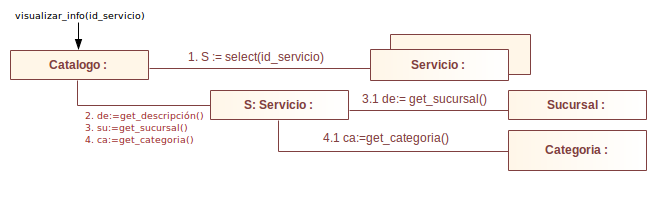
\includegraphics[scale=0.60]{Diagramas/Comunicacion/visualizar_info_servicio.png}
\caption{Diagrama de Comunicación de Caso de Uso Visualizar Información del Servicio }
\label{}
\end{figure}
\newpage
\subsection{Añadir Información}
\begin{center}\begin{figure}[htp]
\centering
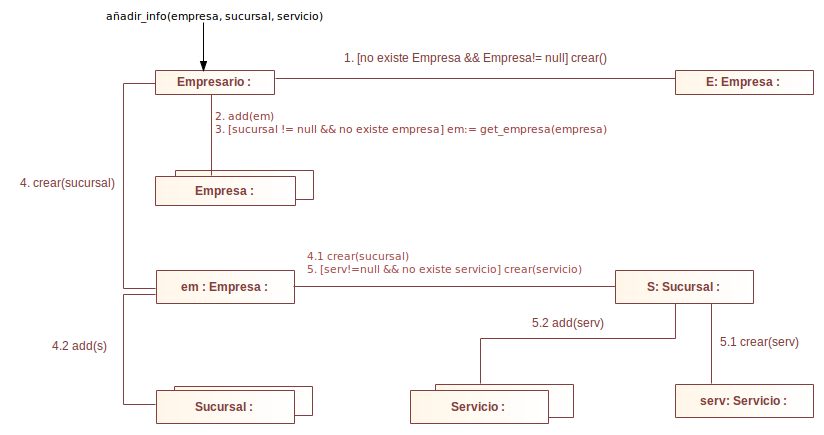
\includegraphics[scale=0.5]{Diagramas/Comunicacion/aniadir_info.png}
\caption{Diagrama de Comunicación de Caso de Uso Añadir Información}
\label{}
\end{figure}\end{center}
\subsection{Buscar de Itinerario}
\begin{center}\begin{figure}[htp]
\centering
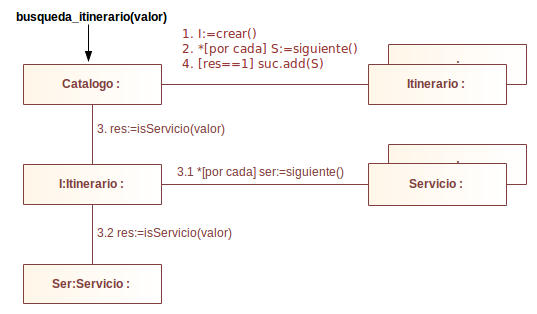
\includegraphics[scale=0.60]{Diagramas/Comunicacion/buscar_itinerario.png}
\caption{Diagrama de Comunicación de Caso de Uso Buscar Itinerario}
\label{}
\end{figure}\end{center}
\newpage
\subsection{Buscar Servicio}
\begin{center}\begin{figure}[htp]
\centering
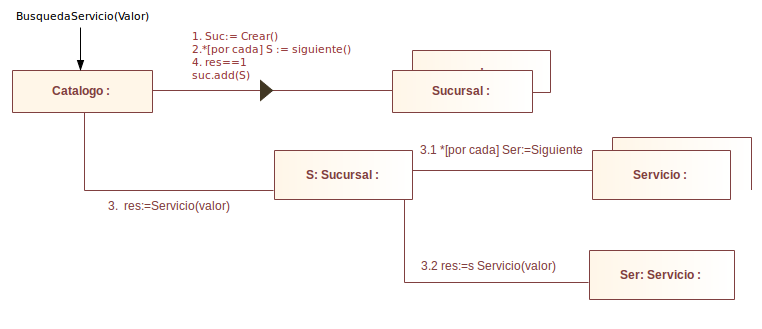
\includegraphics[scale=0.55]{Diagramas/Comunicacion/busqueda_servicio.png}
\caption{Diagrama de Comunicación de Caso de Uso Buscar Servicio}
\label{}
\end{figure}\end{center}
\subsection{Calificar}
\begin{center}\begin{figure}[htp]
\centering
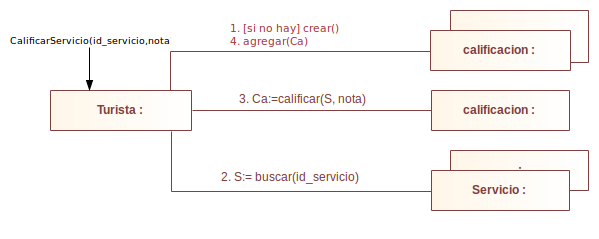
\includegraphics[scale=0.60]{Diagramas/Comunicacion/calificar_servicio.png}
\caption{Diagrama de Comunicación de Caso de Uso Calificar Servicio}
\label{}
\end{figure}\end{center}
\newpage
\subsection{Crear Itinerario}
\begin{center}\begin{figure}[htp]
\centering
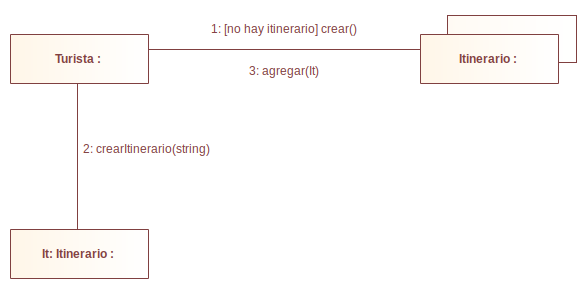
\includegraphics[scale=0.60]{Diagramas/Comunicacion/crear_itinerario.png}
\caption{Diagrama de Comunicación de Caso de Uso Crear Itinerario}
\label{}
\end{figure}\end{center}
\subsection{Visualizar Itinerario}
\begin{center}\begin{figure}[htp]
\centering
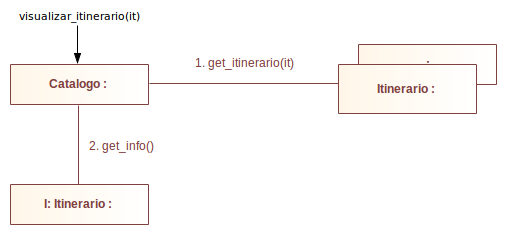
\includegraphics[scale=0.65]{Diagramas/Comunicacion/visualizar_itinerario.png}
\caption{Diagrama de Comunicación de Caso de Uso Visualizar Itinerario}
\label{}
\end{figure}\end{center}
\newpage
%
%Aplicación
%
\section{Aplicación}
La aplicación fue implementada en \emph{Android Studio 2.2.3}
\newpage
\section{Conclusión}
Para la problemática planteada se propuso un sistema computacional que permita el fácil acceso a la información relacionada con los servicios turísticos que actualmente se ubican en la provincia de Arauco. La visualización de este sistema se realizó a través de una aplicación móvil android.\\\\
El diseño de la aplicación contó de varias etapas. En primera instancia generamos una lista de requisitos que debe cumplir la aplicación. Luego identificamos los actores involucrados y los casos de uso del sistema. Para poder crear la base de datos se llevó a cabo el diseño en un diagrama UML que posteriormente se pasó a modelo relacional. Con el modelo relacional terminado fuimos capaces de implementarlo usando MySQL.\\\\Luego de todo lo anterior, dimos paso a la fase de implementación donde - apoyados por los diagramas de secuencia y comunicación - diseñamos la estructura base para programar la versión beta de nuestra aplicación.\\\\Es importante resaltar la gran utilidad que nos permitió el modelo RUP que - entre otros elementos - nos permitió trabajar de manera sistematizada ayudando tanto en la organización como en una implementación limpia y bien documentada. Todo esto nos permitirá continuar evolucionando el Software hacia una \emph{versión estable} más desarrollada.\\\\Si bien en la actualidad existen otros factores que influyen en el desarrollo de un Software (seguridad, manejo de grandes volúmenes de datos, distintos hardware...), en primera etapa los conocimientos aprendidos en el curso resultan ser un buen punto de inicio que potencian nuestro aprendizaje en la Ingeniería de Software. 
.
\newpage
\section{Glosario}
\begin{itemize}
\item \textbf{Punto de interés:} Ubicación especifica en el mapa. 

\item \textbf{Usuario:} Cualquier persona que utiliza la aplicación, ya sea usuario no registrado, turista o empresario. Puede buscar servicios.

\item \textbf{Turista:} Usuario registrado con capacidad de crear, compartir y buscar itinerarios, evaluar servicios? 

\item \textbf{Empresa:} Organización que desarrolla una(s) actividad(es)  turística(s).

\item \textbf{Empresario:} Usuario registrado aparte de turista con capacidad de crear y modificar servicios asociados a él. Es el representante legal de una Empresa.

\item \textbf{Sucursal:} Lugar turístico específico de una Empresa. Tiene un punto de interés.

\item \textbf{Servicio:} Función(es) que desarrolla una sucursal. 

\item \textbf{Categoría:} Tipo de servicio, por ejemplo: gastronómico, turismo vivencia, artesanía, entre otros.

\item \textbf{Sub-Categoría:} Tipo de servicio especifico, por ejemplo de categoría Alojamiento: Hotel, hostal, camping, albergue, entre otros. 

\item \textbf{Itinerario:} Conjunto de puntos de servicios ordenados definidos por un turista.

\item \textbf{Mapa Temático:} Mapa físico de la provincia que incluye iconos de puntos de interés.

\item \textbf{Ruta:} Secuencia de puntos en un mapa que describe la mejor trayectoria entre dos puntos de interés.

\end{itemize}
\end{document}